\subsection{Chromium dimer}

Chromium dimmer has been a challenging problem in quantum chemistry, because large active space is needed to simulate its potential energy curve correct. At the same time, dynamic correlation is also required for a qualitative potential energy curve. \cite{andersson_cr2_1994,roos_multiconfigurational_1995,roos_multiconfigurational_1996,roos_ground_2003,angeli_third-order_2006,muller_large-scale_2009,kurashige_second-order_2011,sharma_multireference_2015}
%Perturbation theory is relatively cheap among methods for dynamic correlation, such as multi-reference couple cluster, multi-reference configuration interaction. It is widely used in the chromium dimmer calculations. 

The CAS(12e,12o), derived from the 3d and 4s atomic orbitals, was widely employed for chrmium dimer calculations.\cite{andersson_cr2_1994,roos_multiconfigurational_1995,roos_multiconfigurational_1996,angeli_third-order_2006,muller_large-scale_2009,sharma_multireference_2015} Both CASPT2\cite{andersson_cr2_1994,roos_multiconfigurational_1995,roos_multiconfigurational_1996} and NEVPT2\cite{angeli_n-electron_2001} based CASSCF(12e,12o) reference function overestimate the dissociation energy of the 3d-3d bond, especially when large basis sets, e.g. g-, h-, or even i- type function, were used.\cite{celani_cipt2_2004,angeli_third-order_2006} And the results from CASPT2(12e,12o) are heavily sensitive to the choice of the zero-order Hamiltonian.\cite{celani_cipt2_2004,ruiperez_complete_2011}
According to NEVPT3 study,\cite{angeli_third-order_2006} the common CAS(12e,12o) wave function is not a good starting reference for the perturbation theory, because the third-order perturbation results in an large fluctuation and an unreasonably curve. DMRG-CASPT2 calculation with a CAS(12e,28o), derived from 3d, 4s, 4p, 4d atomic orbitals, gave potential energy curves close to the experimental one. However, different zero-order Hamiltonians, due to different level shifts in CASPT2, gave quantitatively different results. The difference of $D_e$ with different level shifts was about 0.2eV.
\cite{kurashige_second-order_2011}
DMRG-NEVPT2 is free of intruder state and there is no need add ``level shift'' to change zero-order Hamiltonian. It should be feasible to discribe chromium dimer potential energy curve.

\begin{figure}\label{fig:12o_nevpt2}
  \includegraphics[width=8cm,height=6cm]{application/12o-nevpt2.eps}
  \caption{NEVPT2(12e,12o) potential energy curve with a suite cc-pwcVXZ (X=T,Q,5) basis set}
\end{figure}

A suite of cc-pwcVXZ (X = T,Q,5) basis sets was used in our calculations. No basis set superposition error (BSSE) corrections were applied in the calculations because the BSSE was regarded as small for the large basis sets including h or i-type functions. The X2C Hamiltonian was used to include scalar relativistic effects. 
The energy of isolated atoms was set as zero.
%The symmetry of an isolated atom was set as $C_{\infty v}$, while the dimer's symmetry is set as $D_{\infty h}$. Otherwise, the isolated atom's CAS(6e,9o) will be not consistent with the CAS for the dimer.

For the NEVPT2(12e,12o) potential energy curve of Cr$_2$ in \ref{fig:12o_nevpt2}, larger basis set gives a deeper and worse curve. It agreed with previous studies with atomic natural orbital (ANO) basis sets.\cite{angeli_third-order_2006}
Then the (12e,12o) CAS was extended by adding another set of $\sigma$, $\pi$, $\pi'$, $\delta$, $\delta'$ orbitals and their corresponding anti bond orbitals from external orbitals, forming a CAS(12e,22o). 
DMRG are neccesary here to avoid exponentially increasing computations of FCI.
These additional active orbitals were chosen based on the symmetry and orbital energies; thus their dominant compoents were are from $4p$ and $4d$ orbitals at first. After DMRG-CASSCF orbital optimization ($M=1000$ and there is no frozen core), only $4d$ orbitals component remained. Actually, a 3d double-shell was included in active space, which is reported to greatly increase results of transition metal \cite{andersson_excitation_1992}.
After DMRG-CASSCF orbital optimization, the reference MPS was optimized with $M=4000$. Then the MPS was compressed into a MPS with $M=800$ through ``reverse schedule'', before doing DMRG-NEVPT2 calcualations. To check whether $M=800$ is big enough, the DMRG-NEVPT2 energies with cc-pwcV5Z basis for geometry points near minimum were also calculated with $M=1200$. The difference between curving with $M=800$ and that with $M=1200$ is very small. Finally, the (TZ/QZ/5Z) results were extrapolated to the complete basis set (CBS) limit in exponential formula for DMRG-CASSCF energy and in $l^{-3}$ formula for DMRG-NEVPT2 correction energy.


\begin{figure}\label{fig:5qt_fitting}
  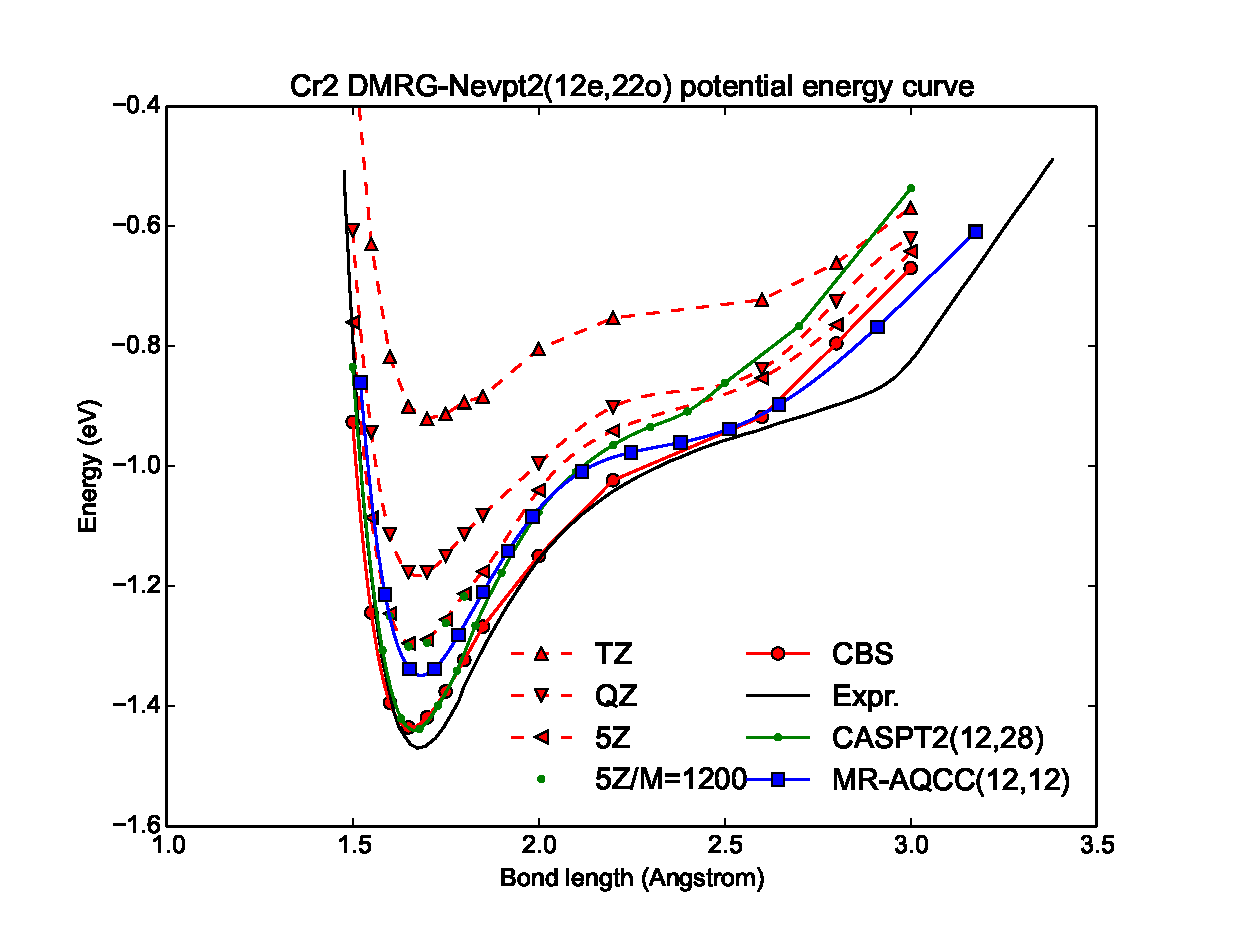
\includegraphics[width=8cm,height=6cm]{application/5qt-fitting.eps}
  \caption{DMRG-NEVPT2(12e,22o)(M=800) potential energy curve with a suite of cc-pwcVXZ (X=T,Q,5) basis set and the complete basis set (CBS) limit. The experimental curve is taken from Ref.~\onlinecite{casey_negative_1993}DMRG-CASCPT2(12e,28o) curve is from Ref.~\onlinecite{kurashige_second-order_2011} and the MR-AQCC(12e,12o) is from Ref.~\onlinecite{muller_large-scale_2009}.}
\end{figure}

Figure \ref{fig:5qt_fitting} shows the potential energy curve with a suite of cc-pwcVXZ (X=T,Q,5) basis set and the complete basis set (CBS) limit. A larger basis set gives a deeper and better curve. The CBS limit potential energy curve agreed with the experimental well, with the exception of the strong bend at about 2.8\AA, where the reliability of the RKR potential in this region has alreadybeen questioned before.\cite{roos_ground_2003}

DMRG-NEVPT2(12e,22o) results were nearly the same with DMRG-CASPT2(12e,28o)\cite{kurashige_second-order_2011} results for the $3d$ bond region. However, for the $4s$ bond (``shoulder'') region, the DMRG-NEVPT2(12e,22o) results were closer to the exerimental one, even though their CAS did not include $4p$ orbitals while DMRG-CASPT2 did. 
It is reasobalbe. Because, in the $4s$ bond region, the correlation is strong, because the $d$ orbitals are not well bonded and nearly degenerate. The Fock operator, monoelectron zero order Hamiltonian in CASPT2, is not good enough. 
The comparision between DMRG-NEVPT2(12e,22o) and DMRG-CASPT2(12e,28o) also indicates, together with the fact that only $4d$ orbitals remained in the active space after orbital optimization, $4d$ orbitals are more important than $4p$ orbitals for the static correlation and the reference function.

%The calcualted $D_e$ is 1.491eV, very close to the experimental value 1.47eV \cite{casey_negative_1993}. However, the calculated bond length is shorter than experimental value. 

\begin{table}
\caption{Spectroscopic Constants for the ground state of Cr$_2$ from different methods}
  \begin{tabular}{cccc}
  \hline
      & $D_e(eV)$ & $R_0($\AA$)$ & $\omega_e$ \\
  \hline
  DMRG-NEVPT2(12e,22o) & 1.436 & 1.656 & 476 \\ 
  DMRG-CASPT2(12e,28o)\footnote{DMRG-CASPT2(12e,28o)/{\bf $g_1$}($M=\infty$) in Ref.~\onlinecite{kurashige_second-order_2011}} & 1.61 & 1.681 & 480 \\
  MR-AQCC(12e,12o)\footnote{Ref.~\onlinecite{muller_large-scale_2009}} & 1.355 & 1.685 & 459 \\
  experiment\footnote{Ref.~\onlinecite{casey_negative_1993}} & 1.47(5) & 1.679 & 480.6(5) \\
  \hline
  \end{tabular}
\end{table}

